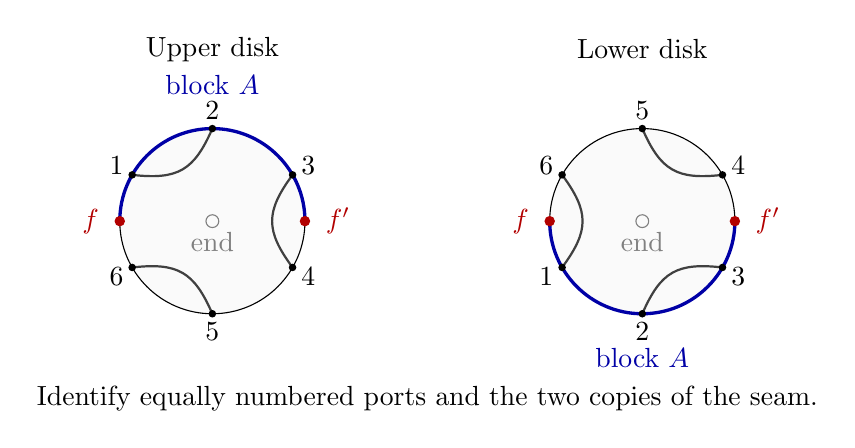
\begin{tikzpicture}[scale=1.05,line cap=round,line join=round,
 arcpath/.style={thick,black!75},seamblock/.style={very thick,blue!65!black}]
\begin{scope}
\draw[fill=gray!4] (0,0) circle (1.12);
\draw[seamblock] (180:1.12) arc (180:0:1.12);
\node[blue!65!black] at (0,1.65) {block $A$};
\node at (0,2.08) {Upper disk};
\draw[arcpath] (150:1.12) .. controls (130:.65) and (110:.65) .. (90:1.12);
\draw[arcpath] (30:1.12) .. controls (10:.65) and (-10:.65) .. (-30:1.12);
\draw[arcpath] (-90:1.12) .. controls (-110:.65) and (-130:.65) .. (-150:1.12);
\foreach \a/\k in {150/1,90/2,30/3,-30/4,-90/5,-150/6}{
 \fill (\a:1.12) circle (1.3pt);\node at (\a:1.34) {$\k$};}
\draw[gray] (0,0) circle (2.2pt);
\node[gray] at (0,-.25) {end};
\fill[red!70!black] (-1.12,0) circle (1.8pt) node[left=4pt] {$f$};
\fill[red!70!black] (1.12,0) circle (1.8pt) node[right=4pt] {$f'$};
\end{scope}
\begin{scope}[xshift=5.2cm]
\draw[fill=gray!4] (0,0) circle (1.12);
\draw[seamblock] (-180:1.12) arc (-180:0:1.12);
\node[blue!65!black] at (0,-1.65) {block $A$};
\node at (0,2.08) {Lower disk};
\draw[arcpath] (-150:1.12) .. controls (-170:.65) and (170:.65) .. (150:1.12);
\draw[arcpath] (-90:1.12) .. controls (-70:.65) and (-50:.65) .. (-30:1.12);
\draw[arcpath] (30:1.12) .. controls (50:.65) and (70:.65) .. (90:1.12);
\foreach \a/\k in {-150/1,-90/2,-30/3,30/4,90/5,150/6}{
 \fill (\a:1.12) circle (1.3pt);\node at (\a:1.34) {$\k$};}
\draw[gray] (0,0) circle (2.2pt);
\node[gray] at (0,-.25) {end};
\fill[red!70!black] (-1.12,0) circle (1.8pt) node[left=4pt] {$f$};
\fill[red!70!black] (1.12,0) circle (1.8pt) node[right=4pt] {$f'$};
\end{scope}
\node at (2.6,-2.14) {Identify equally numbered ports and the two copies of the seam.};
\end{tikzpicture}
